\documentclass[letterpaper, 11pt]{article}

\usepackage{amsmath, amsthm, latexsym, amssymb, graphicx, bold-extra, mathrsfs, frcursive}
\usepackage[pdftex]{color}
\usepackage[T1]{fontenc}

% Simplifies margin settings
\usepackage{geometry}
\geometry{margin=1in}

% Puts list item indicators in bold; makes flush with previous margin
\renewcommand\labelenumi{\bf\theenumi.}
\renewcommand\labelenumii{\bf\theenumii.}
% setlength\leftmargini{1.4em}
\setlength\leftmarginii{1.4em}

% Flexibility for headers and footers
\usepackage{fancyhdr}
\pagestyle{fancyplain}
\fancyhf{} %clear all header and footer fields
\lhead{\bf \small How To Write Fast Numerical Code \hspace*{\fill} Page \thepage}
\headsep 0.2in
\thispagestyle{empty}
\renewcommand{\headrulewidth}{0pt}
\renewcommand{\footrulewidth}{0pt}

\parindent 0in
\parskip 10pt
\setlength{\headheight}{20pt}

\title{ETH Zurich}

\begin{document}

%=======================================

\begin{center}
\Large \bf 263-2300-00: How To Write Fast Numerical Code

\Large \bf Assignment 1: 100 points

\large Submitted by Jinank Jain
\end{center}

\textbf{Solution 1}\\ \\
\textbf{Part a} \\
Processor Manufacturer: Intel \\
Processor Name: i7 \\
Processor Number: 3632QM \\ \\
\textbf{Part b} \\
CPU Logical Cores: 8 \\
CPU Physical Cores: 4 \\ \\ 
\textbf{Part c} \\
CPU Core frequency: 2.2 GHz \\ \\
\textbf{Part d} \\
CPU Maximum Frequency: 3.2 GHz. \\
Yes it does support Intel Turbo Boost Technology (2.0) \\ \\
\textbf{Part e} \\
Tick since my processor belongs to the family of Ivy Bridge Processor. \\ \\
\textbf{Part f-i}
\begin{table}[h!]
\centering
\label{my-label}
\begin{tabular}{|l|l|l|l|}
\hline
OpType         & Latency & Throughput & Gap \\ \hline
Addition       & 3       & 1           &  1   \\ \hline
Multiplication & 5       &  2         & 0.5    \\ \hline
rcp            &  7       &    0.5        &  2   \\ \hline
FMA            & NA      & NA         & NA  \\ \hline
\end{tabular}
\caption{Latency/Throughput/Gap for various operations}
\end{table}

\textbf{Part j} \\
Peak performance: 32 flops/cycle and 102.4 Gflops/sec
\bigskip

\textbf{Solution 2}\\ \\
\textbf{Part a} \\
Appropriate cost function would involve cost of multiplication, additions and divisions individually. One such example could be following:
\begin{center}
$C(n)$ = $C_{add} * N_{add}$ + $C_{mul} * N_{mul}$ + $C_{div} * N_{div}$ + $C_{typecast} * N_{typecast}$
\end{center}
\textbf{Part b}
\begin{center}
$C(n)$ = $C_{add}*(4(n-1)+1)$ + $C_{mul}*(6(n-1)+2)$ + $C_{div}*(2(n-1)+2)$ +  $C_{typecast}*(2(n-1)+2)$ \\
$C(n)$ = $C_{add}*(4n-3)$ + $C_{mul}*(6n-4)$ + $C_{div}*(2n)$ +  $C_{typecast}*(2n)$ \\
$C(n)$ = $flops(n)$ = 14n - 7
\end{center}

\textbf{Solution 3}\\ \\
\begin{figure}[h!]
    \centering
    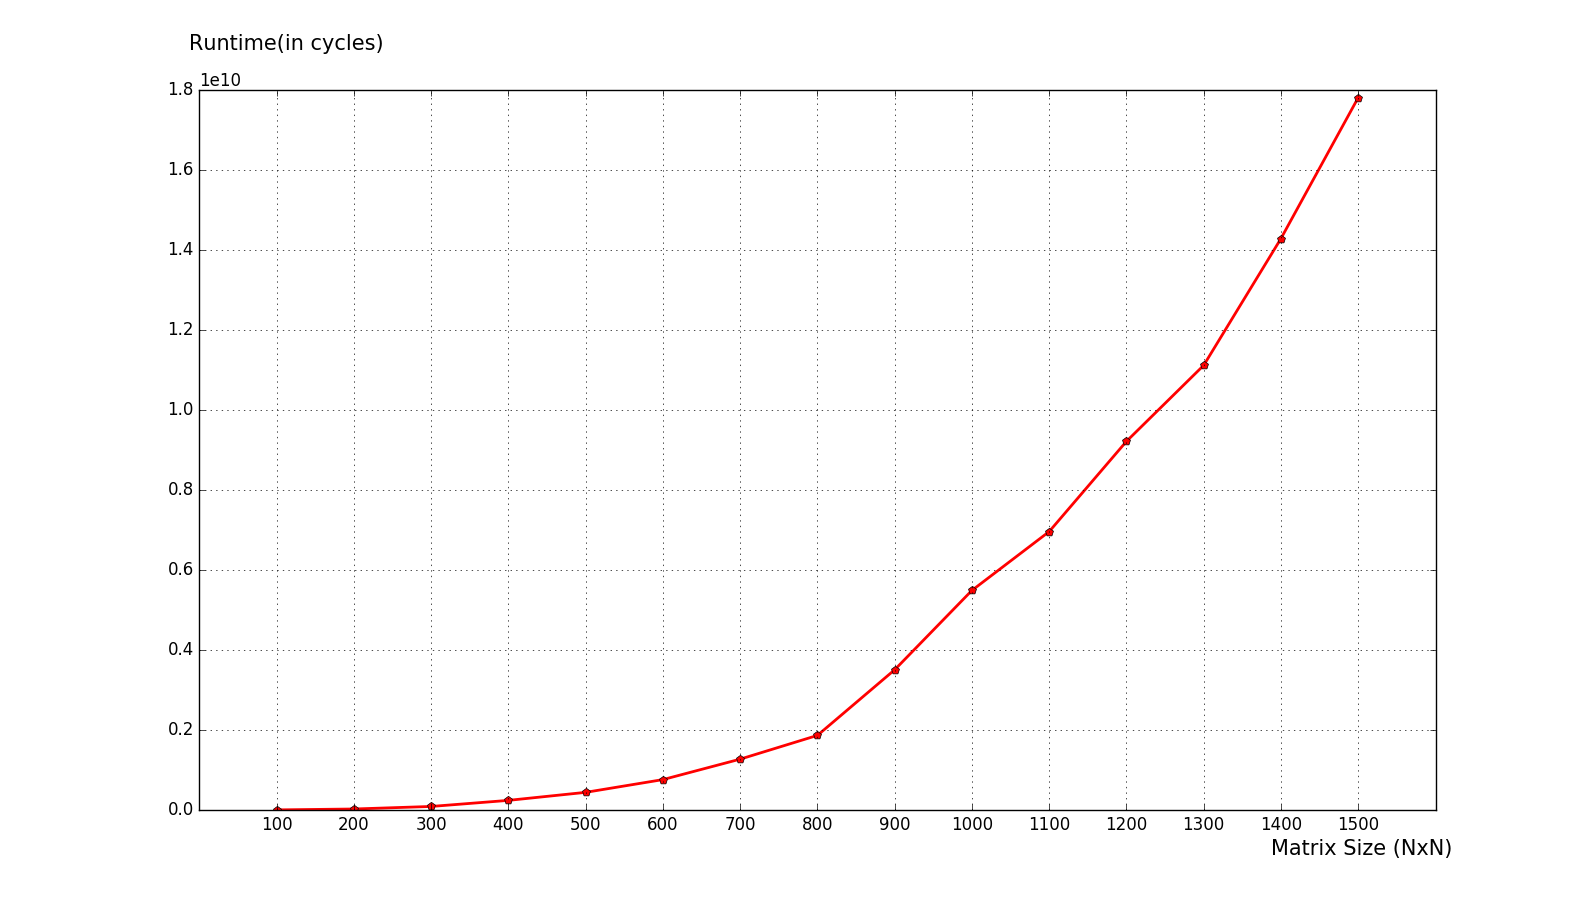
\includegraphics[width=100mm]{sol_3_1}
    \caption{Flow Fairness v/s Per-user fairness}
\end{figure}

\begin{figure}[h!]
    \centering
    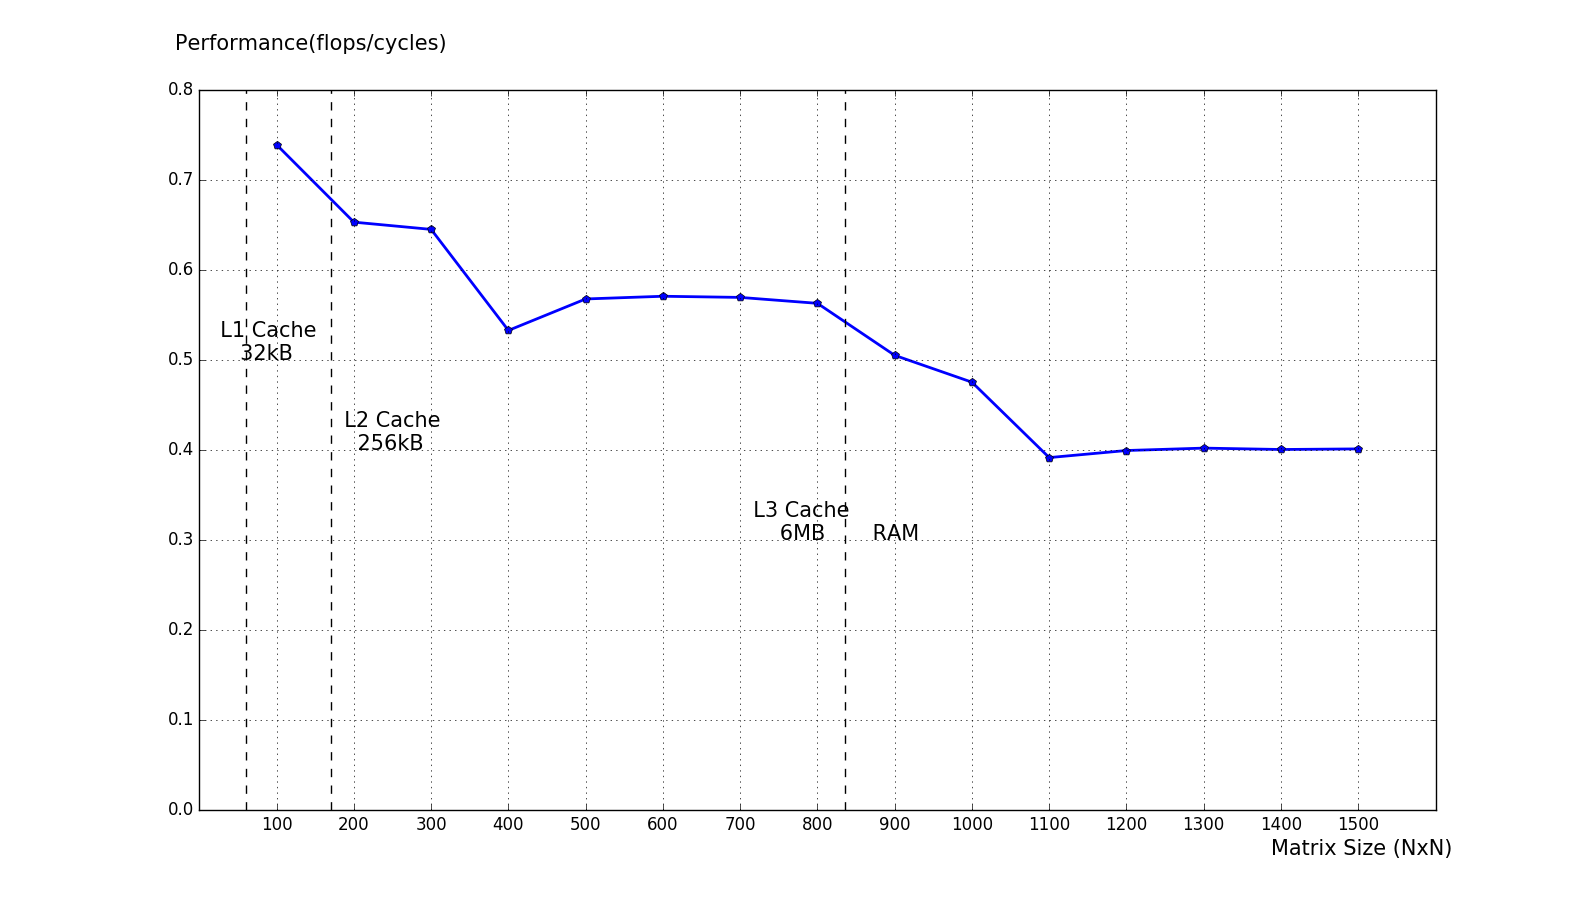
\includegraphics[width=100mm]{sol_3_2}
    \caption{Flow Fairness v/s Per-user fairness}
\end{figure}

\bigskip

\textbf{Solution 4}\\ \\
For example if we look at the paper from Facebook we could find a couple a example due to which traffic would not be rack local:
\begin{itemize}
\item Cache Leader servers won't have rack local traffic as they are achieve cache coherency and in order to do that they need to talk to servers within datacenter or outside datacenter.
\item Cache Follower servers won't have rack local traffic as they are providing data from cache to other servers in the datacenter and that's what was evident from the paper.
\end{itemize}
\bigskip


\textbf{Solution 5}\\ \\
\textbf{Part a}
\begin{itemize}
\item \texttt{artcomp1}: N flops
\item \texttt{artcomp2}: N flops
\item \texttt{artcomp3}: N flops
\end{itemize}
\textbf{Part b}
\begin{itemize}
\item \texttt{artcomp1}: 
\begin{itemize}
\item Flops = N
\item Memory Transfers (floats) $\geq$ 2N
\item Read (bytes) $\geq$ 8N
\item Operational Intensity I(N)  $\leq \frac{1}{8}$ 
\end{itemize}
\item \texttt{artcomp2}: 
\begin{itemize}
\item Flops = N
\item Memory Transfers (floats) $\geq$ 2N
\item Read (bytes) $\geq$ 8N
\item Operational Intensity I(N)  $\leq \frac{1}{8}$ 
\end{itemize}
\item \texttt{artcomp3}: 
\begin{itemize}
\item Flops = N
\item Memory Transfers (floats) $\geq$ 3N
\item Read (bytes) $\geq$ 12N
\item Operational Intensity I(N)  $\leq \frac{1}{12}$ 
\end{itemize}
\end{itemize}
\textbf{Part c} \\
\textbf{i}
\begin{itemize}
\item \texttt{artcomp1}:  N/2
\item \texttt{artcomp2}:  N/2
\item \texttt{artcomp3}:  N/2
\end{itemize}
\textbf{ii}
\begin{itemize}
\item \texttt{artcomp1}:  N/4, N/4, N/2
\item \texttt{artcomp2}:  N/4, N/4, N/2
\item \texttt{artcomp3}:  N/4, 5N/12, 5N/6
\end{itemize}
\bigskip

\clearpage

%=======================================

\end{document}